\section{Empirical Evaluation} \label{sec:evaluation}

Existing methods to discover specific classes on online users are typically validated using a supervised approach, i.e., they rely on expert-generated ground truth.
Such approaches, however, are vulnerable to the subjectivity of the experts, whereby the evaluation would be measuring the fit of the model to the specific experts' own assessment of user instances' relevance. 
In contrast, we follow an unsupervised approach with no a priori knowledge of user relevance. We aim to demonstrate the value of our pipeline in creating a database of online profiles that are ready to be mined, along with examples of candidate user ranking functions.
In this approach, human expertise only comes into play to assess and validate the top-$k$ user lists produced by these functions.
%
We  demonstrate the pipeline in action on a significant set of 25 initial contexts, and define three alternative ranking functions aimed at capturing the empirical notion of  \textit{online activists}.
%
The pipeline is fully implemented in Python using Pandas and public libraries (NetworkX, Selenium) and is available on github\footnote{ \url{https://github.com/flaprimo/twitter-network-analysis}}. 
All experiments are performed on a single Azure node with standard commodity configuration.
Note that we do not focus on system performance as all components operate in near-real time. One exception is  Twitter content harvesting, which is limited by the Twitter API and requires approximately 2 hours per context.

\subsection{Contexts and networks} \label{sec:contexts-selection}
 
We have manually selected 25 contexts within the scope of health awareness campaigns in the UK, all occurring in 2018 and well-characterised using predefined hashtags.
Due to limitations imposed by Twitter on the number of posts that can be retrieved within a time interval, only $200$ tweets were retrieved from each context.
 Table~\ref{tab:contexts} lists the events along with key metrics for their corresponding user-user networks. 
To recall, \textit{assortativity} measures how frequently nodes are likely to connect to other nodes with the same degree ($>0$) or with a different degree ($<0$). 
Negative figures (mean: -0.22, std dev: 0.17) are in line with what is observed on the broader Twitter network~\cite{Fisher2017}.
%
The very small figures for density, defined as $\frac{\#edges }{\mathit{\mathit{\#nodes}} \cdot (\mathit{\#nodes} -1)}$ (mean: 0.004, std dev: 0.002), suggest very few connections exist amongst users within a context. 
This makes it difficult to detect meaningful communities, as described below, thus for some contexts the topological metrics are measured on the entire network as opposed to within each community.
This view is also supported by the average node degree (mean: 2.04, std dev: 0.46) and the ratio of strongly connected components to the number of nodes (mean: 0.98, std. dev. 0.02).

\begin{table}
	\tiny
	\resizebox{\textwidth}{!}{
	    \begin{tabularx}{\textwidth}{|X|P{2.2cm}|P{1.2cm}|P{1cm}|P{1.4cm}|P{1.2cm}|P{1.3cm}|}

\hline
\textbf{Context name} & \textbf{Period (2018)} & \textbf{Nodes} & \textbf{Edges} & \textbf{Density} & \textbf{Avg degree} & \textbf{Assor-tativity} \\ \hline
16 days of action & 11-25 / 12-10 & 396 & 349 & 0.002 & 1.8 & -0.1 \\ \hline
Elf day & 12-03 / 12-12 & 365 & 436 & 0.003 & 2.4 & -0.2 \\ \hline
Dry january & 01-01 / 01-31 & 235 & 234 & 0.004 & 2.0 & -0.3 \\ \hline
Cervical cancer prevention week & 01-21 / 01-27 & 209 & 192 & 0.004 & 1.8 & -0.1 \\ \hline
Time to talk day & 02-06 / 02-07 & 268 & 231 & 0.003 & 1.7 & -0.2 \\ \hline
Eating disorder awareness week & 02-25 / 03-03 & 256 & 241 & 0.004 & 1.9 & -0.2 \\ \hline
Rare disease day & 02-28 / 03-01 & 294 & 206 & 0.002 & 1.4 & -0.2 \\ \hline
Ovarian cancer awareness month & 03-01 / 03-31 & 215 & 202 & 0.004 & 1.9 & -0.4 \\ \hline
Nutrition and hydration week & 03-11 / 03-17 & 273 & 326 & 0.004 & 2.4 & -0.3 \\ \hline
Brain awareness week & 03-11 / 03-17 & 307 & 281 & 0.003 & 1.8 & -0.1 \\ \hline
No smoking day & 03-13 / 03-14 & 254 & 219 & 0.003 & 1.7 & -0.3 \\ \hline
Epilepsy awareness purple day & 03-26 / 03-27 & 306 & 252 & 0.003 & 1.6 & -0.2 \\ \hline
Experience of care week & 04-23 / 04-27 & 176 & 196 & 0.006 & 2.2 & -0.1 \\ \hline
Brain injury week & 05-01 / 05-31 & 238 & 306 & 0.005 & 2.6 & -0.1 \\ \hline
Mental health awareness week & 05-14 / 05-20 & 268 & 245 & 0.003 & 1.8 & -0.5 \\ \hline
Dementia action week & 05-21 / 05-31 & 300 & 300 & 0.003 & 2.0 & -0.0 \\ \hline
Mnd awareness month & 06-01 / 06-30 & 141 & 234 & 0.012 & 3.3 & -0.3 \\ \hline
Wear purple for jia & 06-01 / 06-30 & 165 & 245 & 0.009 & 3.0 & -0.5 \\ \hline
Carers week & 06-11 / 06-17 & 270 & 277 & 0.004 & 2.1 & 0.0 \\ \hline
National dementia carers & 09-09 / 09-10 & 184 & 177 & 0.005 & 1.9 & -0.2 \\ \hline
Mens health week & 06-11 / 06-17 & 264 & 214 & 0.003 & 1.6 & -0.2 \\ \hline
Stress awareness day & 11-07 / 11-08 & 293 & 209 & 0.002 & 1.4 & -0.2 \\ \hline
National dyslexia week & 10-01 / 10-07 & 229 & 235 & 0.004 & 2.1 & -0.2 \\ \hline
Ocd awareness week & 10-07 / 10-13 & 202 & 193 & 0.005 & 1.9 & -0.6 \\ \hline
Jeans for genes day & 09-21 / 09-22 & 246 & 325 & 0.005 & 2.6 & -0.2 \\ \hline

\end{tabularx}

	}
	\caption{List of contexts used in the experiments along with network metrics.}
	\label{tab:contexts}
\vspace{-20pt}
\end{table}


\subsection{Communities}  \label{sec:communities-eval}

 \demon~and \infomap~ produce significantly different communities in each network. 
%
\demon~identifies communities in only 48\% of the networks, with an average of only 1.92 communities per network and 
a slightly negative  (-0.28) average assortativity  per community, in line with the average for their parent networks.
%
Only the users who belong to one of those communities, about 6\%, are added to the database.
%
For the remaining 52\% of networks where no communities are detected, users' in-degrees are calculated using the entire network, and all users are added to the database, 
for a total of 3,570 users being added to the database in our experiments using \demon.

In contrast, \infomap~provides meaningful communities for all networks.
Those with fewer than 3 users are discarded, leaving  18.88 communities per network on average, with 8.5 users per community on average.
% The rightmost column in Table~\ref{tab:contexts} reports the number of communities normalised by the size of the network, where a  contains . 
When using Infomap, 3,567 users were added to the database (on average 253 users per network).
The average assortativity across all communities is again slightly negative (-0.43).
%
Table~\ref{tab:demon-vs-infomap} compares the two approaches on the key metrics just discussed. On the basis of this comparison, we recommend using \infomap, which we have used for  our evaluation.

\begin{table}
	\vspace{-10pt}
		\footnotesize
	\resizebox{\textwidth}{!}{
	    \begin{tabularx}{\textwidth}{|X|P{1.7cm}|P{1.7cm}|}
\hline
\textbf{Metric} & \textbf{\demon} & \textbf{\infomap} \\ \hline
Fraction of networks with null communities & 0.52 & 0.0 \\ \hline
Number of communities per context (avg) & 1.92 & 18.88 \\ \hline
Fraction of network users added to the DB  (avg) & 0.06 & 0.59 \\ \hline
Fraction of repeat users  added to the DB across networks & 0.28 & 0.37 \\ \hline
\end{tabularx}
	}
	\caption{Comparing \demon~to \infomap~for community detection.}
	\label{tab:demon-vs-infomap}
	\vspace{-20pt}
\end{table}

\subsection{Users discovery}  \label{sec:users}

Repeat users who appear in multiple contexts are particularly interesting as they provide a stronger signal. 
Out of the total 3,567 users, 160 of those appear at least in two of the 25 contexts.
After community detection, only 61 of these users are still seen as repeat users,
while the remaining 99 are either removed altogether, or they only appear once.
Of the 61, 57 appear twice, 2 appear three times, and 2 appear four times. 
Thus, only 1.6\% of users appear more than once when communities with more than 3 users are considered, compared to the overall 4.5\% of overall repeat users.
%
Table~\ref{tab:repeat-users} reports the top-10 repeat users along with their \textit{Follower Rank}, and Fig.~\ref{fig:repeat-users-frequency} shows the number of repeat users per context.
As the table is sorted by number of occurrences then by \textit{Follower Rank}, an indication of popularity,  it is not surprising to find that top users include well-known names such as Mr. Hunt, who at the time of the events was Secretary of State for Health and Social Care in the UK, with $FR =1$, and a number of associations and foundations active in the public healthcare space.
More interesting are perhaps non-repeat users who emerge when ad hoc ranking is applied to the database, as we illustrate next.

\begin{table}[htb]
	\centering
	\footnotesize
	\resizebox{\textwidth}{!}{
		\begin{tabularx}{\textwidth}{|p{2.5cm}|X|P{2.4cm}|P{2.4cm}|}
\hline
\textbf{Username} & \textbf{Name} & \textbf{Follower rank} & \textbf{Participations} \\ \hline
alzheimerssoc & Alzheimer's Society & 0.99 & 4 \\ \hline
dementiauk & Dementia UK & 0.98 & 4 \\ \hline
mentalhealth & Mental Health Fdn & 0.97 & 3 \\ \hline
colesmillerllp & Coles Miller LLP & 0.65 & 3 \\ \hline
rdash\_nhs & RDaSH NHS FT & 0.88 & 2 \\ \hline
alzsocseengland & Alzheimer's Society - South ... & 0.64 & 2 \\ \hline
jeremy\_hunt & Jeremy Hunt & 1.0 & 2 \\ \hline
nhsengland & NHS England & 0.99 & 2 \\ \hline
carersuk & Carers UK & 0.95 & 2 \\ \hline
mndassoc & MND Association & 0.64 & 2 \\ \hline
\end{tabularx}
	}
	\caption{Top-10 repeat users, amongst those who belong to a community.}
	\label{tab:repeat-users}
	\vspace{-20pt}
\end{table}

\begin{figure*}[htb]
	\centering
	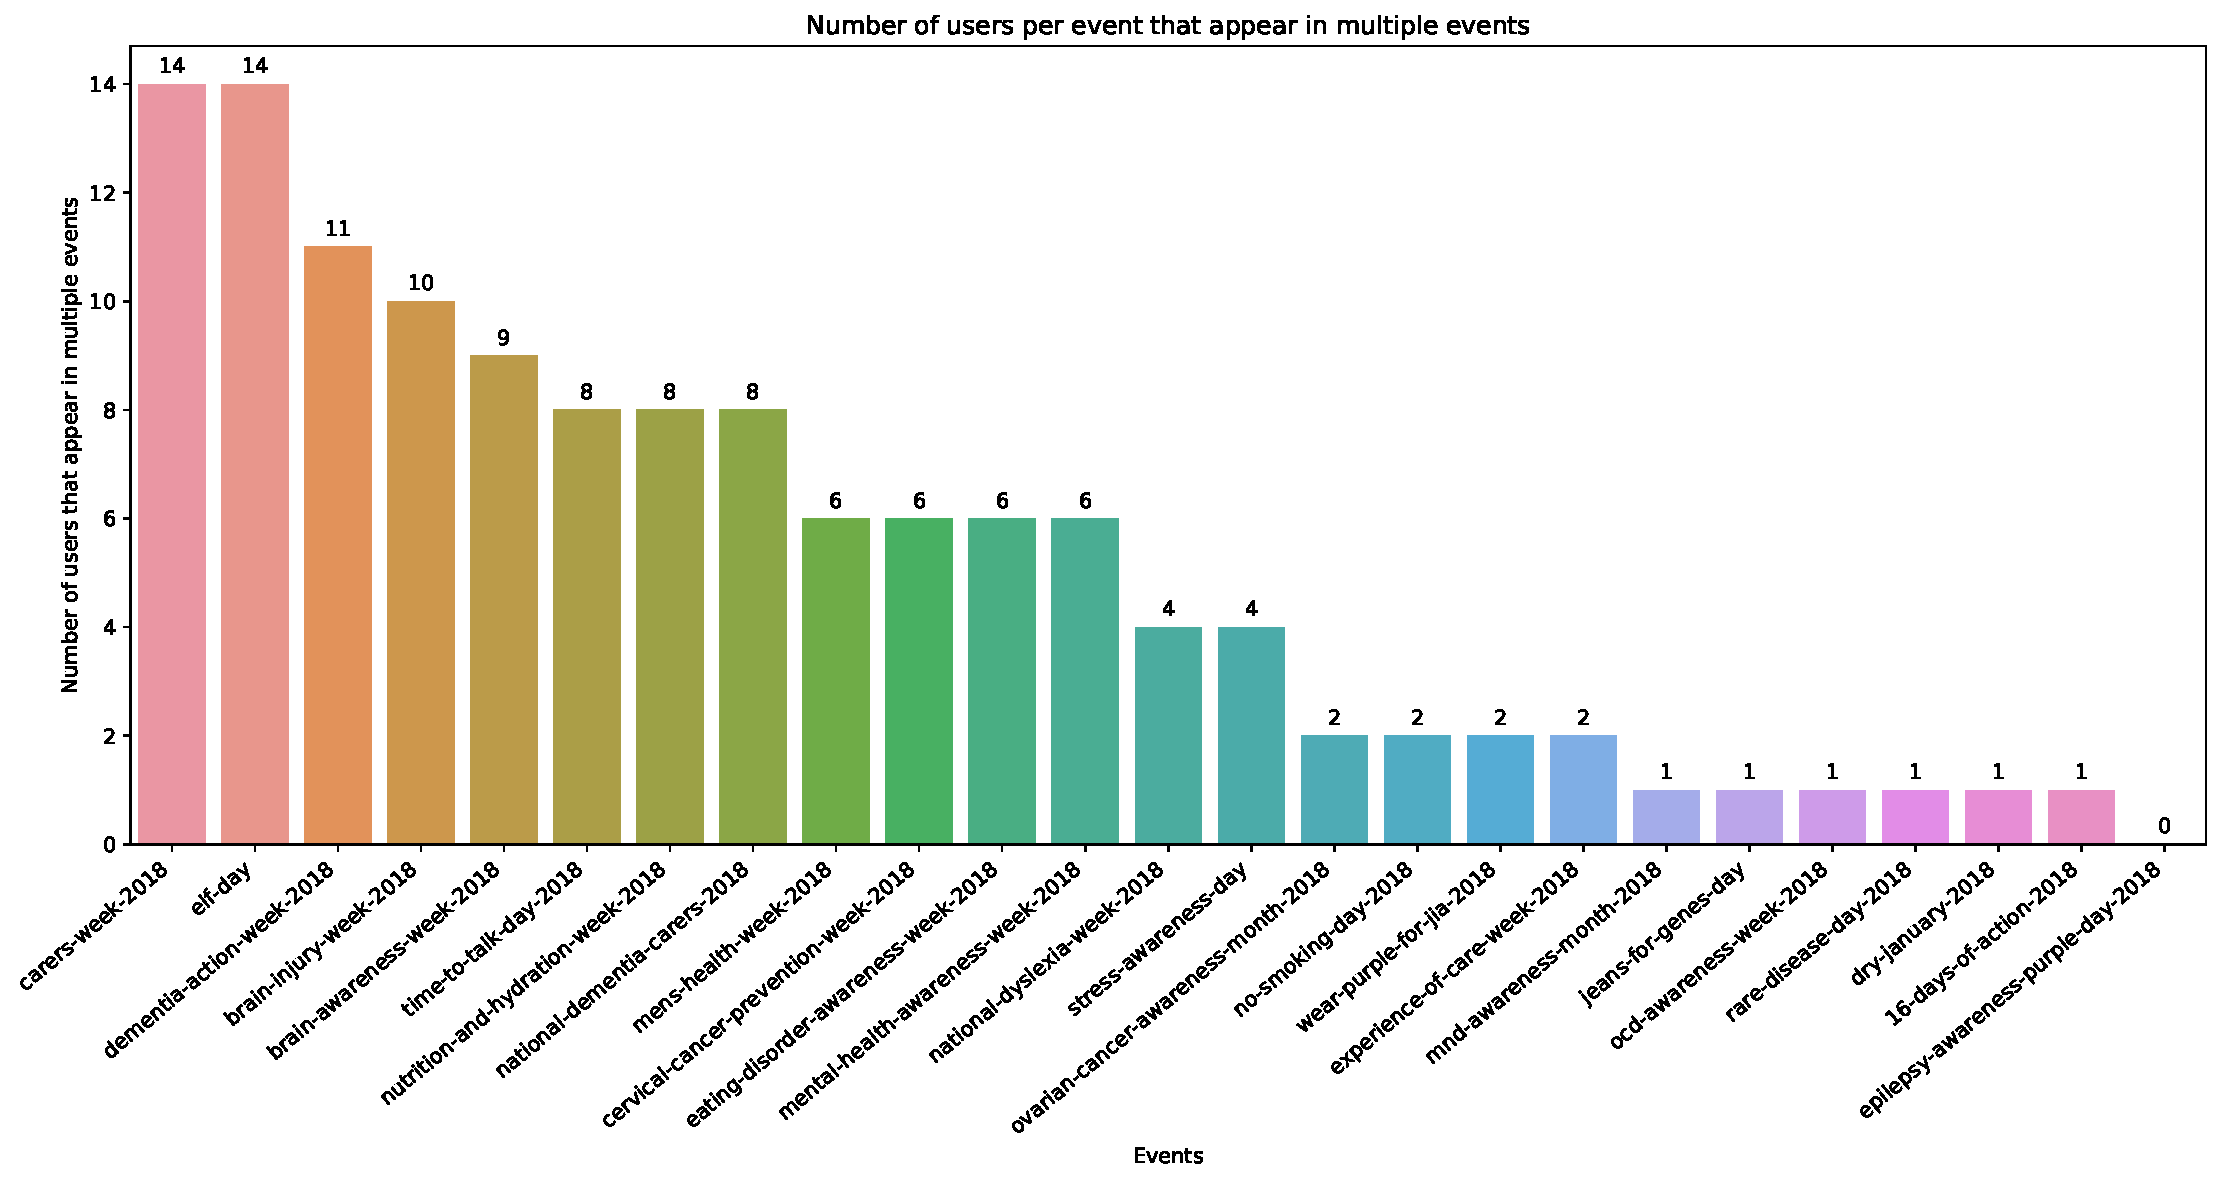
\includegraphics[width=1.2\textwidth]{figures/repeat-users-frequency}
	\caption{Number of repeat users for each context}
	\label{fig:repeat-users-frequency}
\end{figure*}

\vspace{-10pt}
\subsection{Users ranking} \label{sec:ranking}
%\vspace{-10pt}

To demonstrate the potential value of the database, albeit on a small scale, we have tested three user ranking functions.
As mentioned, the aim of this exercise is to provide an objective grounding for engaging with experts on finding suitable operational definitions for specific user profiles. We consider good functions those that privilege individuals over organisations or business.
%
\begin{table}
			\vspace{-20pt}
	\centering
	\footnotesize
	\resizebox{\textwidth}{!}{
		% \begin{tabular}{P{0.6cm}|p{2.3cm}|P{1.4cm}|P{1.8cm}|p{2.3cm}|P{1.4cm}|P{1.8cm}|}

% \cline{2-7}
% \multicolumn{1}{l|}{} & \multicolumn{3}{c|}{\textbf{Ranking 1}} & \multicolumn{3}{c|}{\textbf{Ranking 2}} \\ \hline
% \multicolumn{1}{|c|}{\textbf{\#}} & \textbf{User} & \textbf{On-topic} & \textbf{Individual} & \textbf{User} & \textbf{On-topic} & \textbf{Individual} \\ \hline
% \multicolumn{1}{|c|}{1} & homesnutrition & X &  & johnneustadt & X & X \\ \hline
% \multicolumn{1}{|c|}{2} & ficajones & X & X & jo\_millar27 & X & X \\ \hline
% \multicolumn{1}{|c|}{3} & helenvweaver & X & X & hatchbrenner &  &  \\ \hline
% \multicolumn{1}{|c|}{4} & spriggsnutri & X &  & nchawkes & X & X \\ \hline
% \multicolumn{1}{|c|}{5} & critcarelthtr & X &  & moz0373runner & X & X \\ \hline
% \multicolumn{1}{|c|}{6} & danielleroisin\_ & X & X & aimsonhealth & X & X \\ \hline
% \multicolumn{1}{|c|}{7} & mynameisandyj & X & X & wordsharkv5 &  & X \\ \hline
% \multicolumn{1}{|c|}{8} & fionaliu92 & X & X & fullcircle\_play & X &  \\ \hline
% \multicolumn{1}{|c|}{9} & ldpartnership & X &  & qsprivatehealth & X &  \\ \hline
% \multicolumn{1}{|c|}{10} & milaestevam1 &  & X & socialissp &  &  \\ \hline

% \end{tabular}

\begin{tabular}{P{0.6cm}|p{2.3cm}|P{1.4cm}|P{1.8cm}|p{2.3cm}|P{1.4cm}|P{1.8cm}|p{2.3cm}|P{1.4cm}|P{1.8cm}|}

\cline{2-10}
\multicolumn{1}{l|}{} & \multicolumn{3}{c|}{\textbf{Ranking 1}} & \multicolumn{3}{c|}{\textbf{Ranking 2}} & \multicolumn{3}{c|}{\textbf{Ranking 3}} \\ \hline
\multicolumn{1}{|c|}{\#} & \textbf{User} & \textbf{On-topic} & \textbf{Individual} & \textbf{User} & \textbf{On-topic} & \textbf{Individual} & \textbf{User} & \textbf{On-topic} & \textbf{Individual} \\ \hline
\multicolumn{1}{|c|}{1} & homesnutrition & X &  & johnneustadt & X & X & johnneustadt &  & X \\ \hline
\multicolumn{1}{|c|}{2} & ficajones & X & X & jo\_millar27 & X & X & solutions777 & X & X \\ \hline
\multicolumn{1}{|c|}{3} & helenvweaver & X & X & hatchbrenner &  &  & kingste29344921 & X & X \\ \hline
\multicolumn{1}{|c|}{4} & spriggsnutri & X &  & nchawkes & X & X & daisylu1964 & X &  \\ \hline
\multicolumn{1}{|c|}{5} & critcarelthtr & X &  & moz0373runner & X & X & zakariamarsli & X & X \\ \hline
\multicolumn{1}{|c|}{6} & danielleroisin\_ & X & X & aimsonhealth & X & X & meowaaaaaa & X &  \\ \hline
\multicolumn{1}{|c|}{7} & mynameisandyj & X & X & wordsharkv5 &  & X & vecta67 & X &  \\ \hline
\multicolumn{1}{|c|}{8} & fionaliu92 & X & X & fullcircle\_play & X &  & cosfordfamily1 & X & X \\ \hline
\multicolumn{1}{|c|}{9} & ldpartnership & X &  & qsprivatehealth & X &  & hayleycorriganx & X &  \\ \hline
\multicolumn{1}{|c|}{10} & milaestevam1 &  & X & socialissp &  &  & jhbrasfie & X &  \\ \hline

\end{tabular}
	}
	\caption{Top-10 ranked users for ranking functions (\ref{eq:rank1}) and (\ref{eq:rank2}) and (\ref{eq:rank3}), with indication of whether the user is on-topic/off-topic and individual vs association.}
	\label{tab:rank1}
	\vspace{-30pt}
\end{table}
%

\begin{align}
\textit{Ranking 1:} ~ \mathit{R1}(u) & = \frac{1}{\sum_{u \in C} \mathit{IC}(u) + 1} \cdot \sum_{u \in C} \mathit{TF}(u) \label{eq:rank1} \\
\textit{Ranking 2:} ~ \mathit{R2}(u) & = \lvert \mathit{FR}(u) - 1 \rvert \cdot \left(\sum_{u \in C} \mathit{TA}(U) + \sum_{u \in C} \mathit{IC}(U)\right) \label{eq:rank2} \\
\textit{Ranking 3:} ~ \mathit{R3}(u) & = \lvert \mathit{FR}(u) - 1 \rvert \cdot \left(\sum_{u \in C} \mathit{TA}(U) + \frac{1}{\sum_{u \in C} \mathit{IC}(U) + 1}\right) \label{eq:rank3}
\end{align}
%
Function (\ref{eq:rank1}) is designed to promote users who are at the ``fringe'' of their community, while giving credit to generic on-topic activities during the contexts. 
To achieve this, \textit{Topical Focus} $\mathit{TF}$ is used as a positive contribution, while a large in-degree $\mathit{IC}$ reduces the score.
%
In contrast, function (\ref{eq:rank2}) penalises user popularity, i.e., by using the complement of \textit{Follower Rank} $\mathit{FR}$, while rewarding prominence inside communities (in-degree $\mathit{IC}$) and information spreading by also considering shared links (\textit{Topical Attachment} $\mathit{TA}$).
%
Function (\ref{eq:rank3}) combines idea from both (\ref{eq:rank21}) and  (\ref{eq:rank1}).

The top-10 users for each ranking are reported in Tab.~\ref{tab:rank1}. To appreciate the effects of these functions, we have manually labelled the top-100 user profiles for each of the rankings, using a broad type classification as \textit{individuals} as opposed to \textit{institutional players} (associations, public bodies), or \textit{professionals}. 
%
The fractions of on-topic users are 86\%, 83\%, and 38\% for (\ref{eq:rank1}), (\ref{eq:rank2}), and (\ref{eq:rank2}) respectively.
Importantly, (\ref{eq:rank3}) identifies more individuals than institutions and professionals (96\%) than (\ref{eq:rank2}) and (\ref{eq:rank3}), both at 33\%, among in-topic users.
%
%The fractions of on-topic users are 90\%, 70\%, and \hl{X\%} respectively.
Also, repeat users are rewarded in both rankings. Users with $\mathit{FR}(u) = 0$ and $\mathit{min\_max(\lvert Tweets (u)\rvert) < 0.005}$ are considered not active and have been assigned lowest score.
Fig.~\ref{fig:ranks-distribution} shows the distribution of user types within the top-100 users for each of the three rankings, broken down into 10 users bins. We can see that individuals dominate in (\ref{eq:rank3}), and are fewer but  emerge earlier in the ranks when (\ref{eq:rank2}) is used.
We plan to conduct user studies to establish useful analytics to be incorporated into our framework. 
\begin{figure}[htb]
	\centering
	\begin{subfigure}{.49\textwidth}
		\centering
		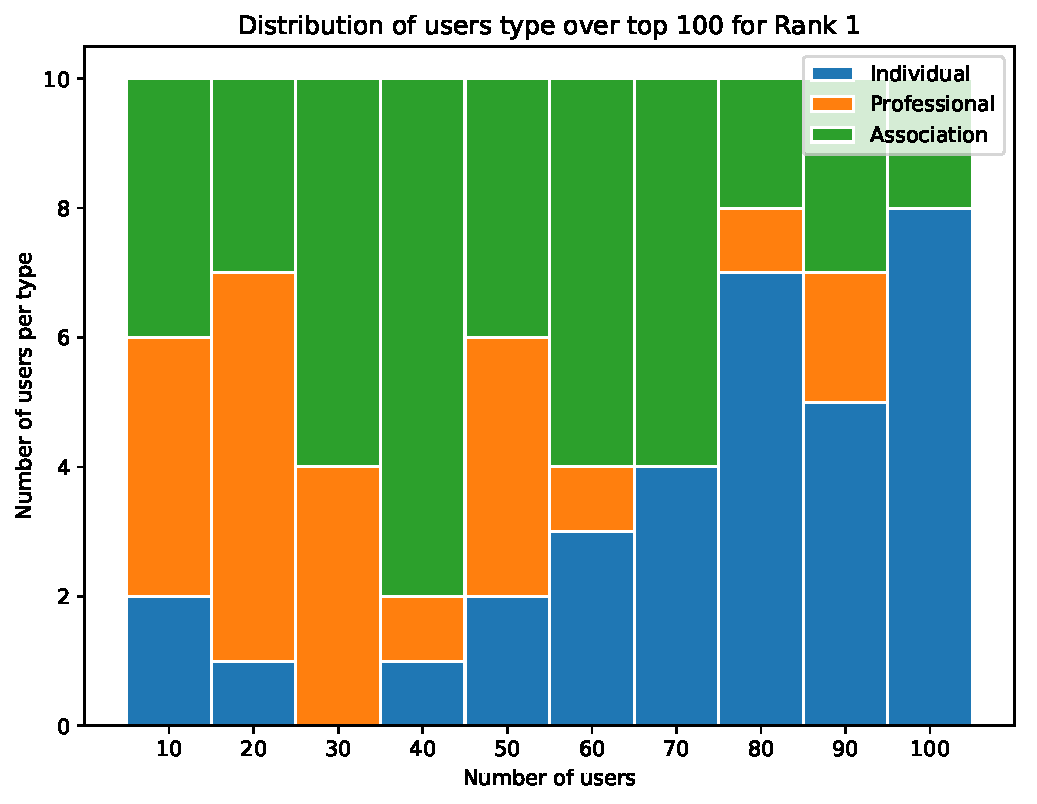
\includegraphics[width=\textwidth]{figures/rank1-distribution.pdf}
		\caption{Rank 1: 33 are individuals, 23 are professionals, 44 are associations}
		\label{fig:rank1-distribution}
	\end{subfigure}
	\hfill%
	\begin{subfigure}{.49\textwidth}
		\centering
		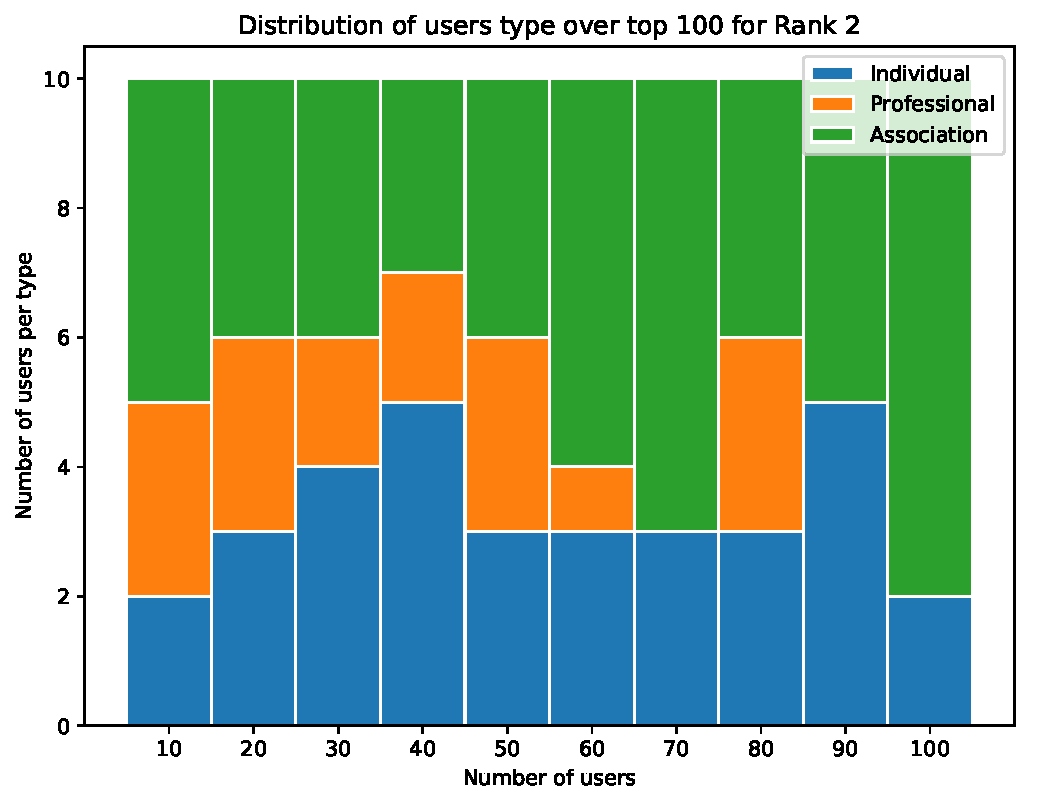
\includegraphics[width=1\textwidth]{figures/rank2-distribution.pdf}
		\caption{Rank 2: 33 are individuals, 17 are professionals, 50 are associations}
		\label{fig:rank2-distribution}
	\end{subfigure}
	\hfill%
	\begin{subfigure}{.49\textwidth}
		\centering
		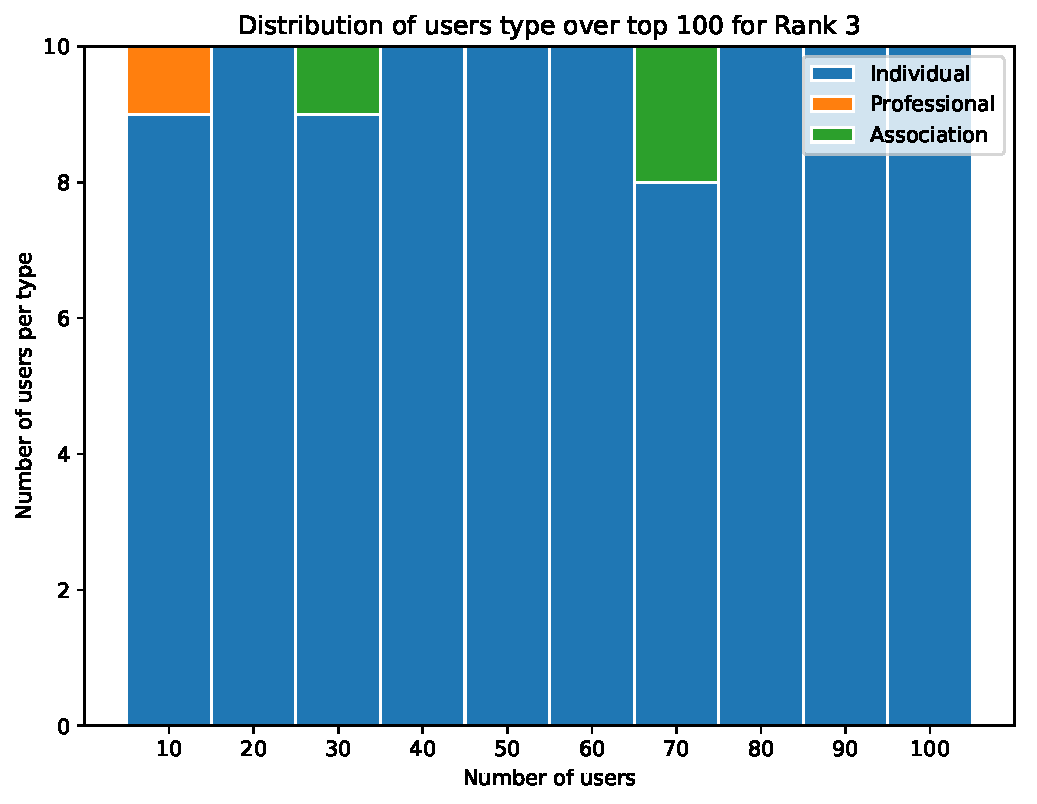
\includegraphics[width=1\textwidth]{figures/rank3-distribution.pdf}
		\caption{Rank 3: 96 are individuals, 1 are professionals, 3 are associations}
		\label{fig:rank3-distribution}
	\end{subfigure}
	\caption{Distribution of user types for top-100 users and for each ranking function.}
	\label{fig:ranks-distribution}
\end{figure}
%